\documentclass[10pt]{standalone}
\usepackage[sc]{mathpazo}
\usepackage{commands}
\renewcommand{\phi}{\varphi}

\begin{document}
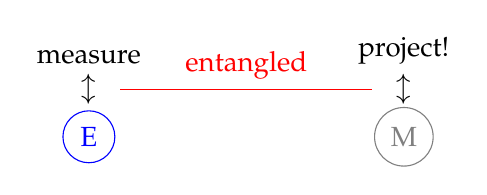
\begin{tikzpicture}[scale=2]
    \node[circle, draw, blue] (E) at (0, 0) {E};
    \node[circle, draw, gray] (M) at (2, 0) {M};
    \node[] at (0, 0.3) {$\ket{\updownarrow}$};
    \node[] at (2, 0.3) {$\ket{\updownarrow}$};
    \draw[red] (0.2, 0.3) -- (1.8, 0.3);
    \node[red, above] at (1, 0.3) {entangled};
    \node[above] at (0, 0.4) {measure};
    \node[above] at (2, 0.4) {project!};
\end{tikzpicture}
\end{document}